\documentclass[tikz,border=6pt]{standalone}
\usetikzlibrary{arrows.meta,positioning,calc}
\usepackage{amsmath}
\usepackage[T1]{fontenc}
\usepackage{lmodern}

\begin{document}
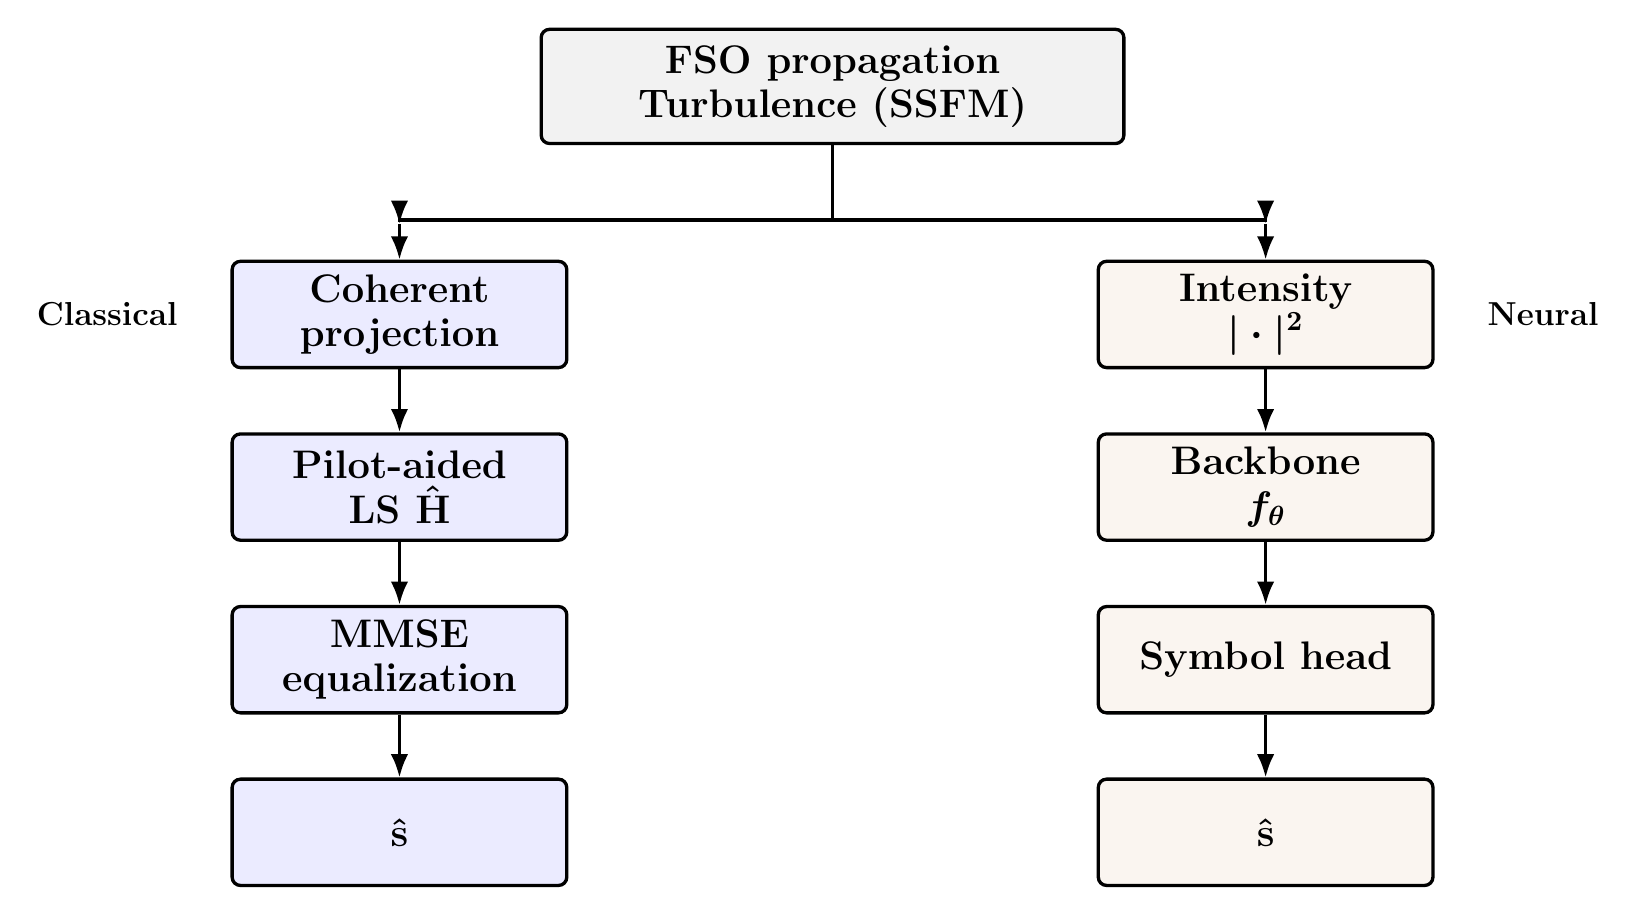
\begin{tikzpicture}[
  >=Latex,
  font=\sffamily,
  line/.style={-Latex, very thick},
  topbox/.style={
    draw, rounded corners=3pt, very thick, align=center,
    minimum width=7.4cm, minimum height=1.45cm, fill=gray!10,
    font=\bfseries\boldmath\fontsize{14}{16}\selectfont
  },
  cbox/.style={
    draw, rounded corners=3pt, very thick, align=center,
    minimum width=4.25cm, minimum height=1.35cm, fill=blue!8,
    font=\bfseries\boldmath\fontsize{14}{16}\selectfont
  },
  nbox/.style={
    draw, rounded corners=3pt, very thick, align=center,
    minimum width=4.25cm, minimum height=1.35cm, fill=brown!8,
    font=\bfseries\boldmath\fontsize{14}{16}\selectfont
  },
  side/.style={font=\bfseries\fontsize{12}{14}\selectfont}
]

% Top node
\node[topbox] (top) {FSO propagation\\Turbulence (SSFM)};

% Branch root coordinates
\coordinate (splitL) at ($(top.south)+(-5.5cm,-1.00cm)$);
\coordinate (splitR) at ($(top.south)+( 5.5cm,-1.00cm)$);

% Branch boxes: classical
\node[cbox] (c1) at ($(splitL)+(0,-1.15cm)$) {Coherent\\projection};
\node[cbox, below=0.8cm of c1] (c2) {Pilot-aided\\LS $\hat{\mathbf{H}}$};
\node[cbox, below=0.8cm of c2] (c3) {MMSE\\equalization};
\node[cbox, below=0.8cm of c3] (c4) {$\hat{\mathbf{s}}$};

% Branch boxes: neural
\node[nbox] (n1) at ($(splitR)+(0,-1.15cm)$) {Intensity\\$|\cdot|^2$};
\node[nbox, below=0.8cm of n1] (n2) {Backbone\\$f_{\theta}$};
\node[nbox, below=0.8cm of n2] (n3) {Symbol head};
\node[nbox, below=0.8cm of n3] (n4) {$\hat{\mathbf{s}}$};

% Trunk and branch connectors
\draw[line] (top.south) -- ++(0,-0.95cm) -| (splitL);
\draw[line] (top.south) -- ++(0,-0.95cm) -| (splitR);
\draw[line] (splitL) -- (c1.north);
\draw[line] (splitR) -- (n1.north);

% Vertical flows
\draw[line] (c1) -- (c2);
\draw[line] (c2) -- (c3);
\draw[line] (c3) -- (c4);
\draw[line] (n1) -- (n2);
\draw[line] (n2) -- (n3);
\draw[line] (n3) -- (n4);

% Side labels
\node[side, left=0.55cm of c1] {Classical};
\node[side, right=0.55cm of n1] {Neural};

\end{tikzpicture}
\end{document}
